\documentclass[a4paper, 12pt]{article}
\usepackage[T1]{fontenc}
\usepackage[utf8]{inputenc}
\usepackage{graphicx}
\usepackage{hyperref}
\usepackage{tabularx}
\usepackage{stfloats}
\usepackage{url}
\usepackage{subfigure}
\usepackage{amsmath}

\hypersetup{
    pdfborder={0 0 0}
}

\newcommand{\risk}[4]{
    \item \textbf{Risk:} #1
    \begin{itemize}
        \item \textbf{Probability:} #2
        \item \textbf{Damage:} #3
        \item \textbf{How to deal with it:} #4
    \end{itemize}
}

\newcommand{\cost}[7] {
    \def\tempa{#1}
    \def\tempb{#2}
    \def\tempc{#3}
    \def\tempd{#4}
    \def\tempe{#5}
    \def\tempf{#6}
    \def\tempg{#7}
    \runcost
}

\newcommand{\ssc}[2][c]{%
  \begin{tabular}[#1]{@{}c@{}}#2\end{tabular}}

\newcommand{\runcost}[8]{
\paragraph{\tempa} \tempb \\
#8 \\ 
\begin{table}[h]\centering \hspace*{-1.5cm} \small
\begin{tabular}{| p{2cm} | p{2cm} | p{2cm} | p{2cm} | p{2cm} | p{2cm} | p{2cm} |} \hline
\ssc{\\ \textbf{\tempa} \\ \textbf{Descriptors} } & \tempc & \tempd & \tempe & \tempf & \tempg & #1\\ \hline
\ssc{ \textbf{Rating} \\ \textbf{Levels} }  & \textbf{Very Low} & \textbf{Low} & \textbf{Nominal} & \textbf{High} & \textbf{Very High} & \textbf{Extra High} \\ \hline
\ssc{ \textbf{Effort}\\ \textbf{Multipliers}} & #2 & #3 & #4 & #5 & #6 & #7 \\ \hline 
\end{tabular}
\caption{\tempa~Descriptors}
\label{cost:#1}
\end{table}
}

\newcommand{\scost}[9]{
\paragraph{#1} #2 \\
#9 \\ 
\begin{table}[h]\centering \hspace*{-1.5cm} \small
\begin{tabular}{| p{2cm} | p{2cm} | p{2cm} | p{2cm} | p{2cm} | p{2cm} | p{2cm} |} \hline
    \ssc{ \textbf{Rating} \\ \textbf{Levels} }  & \textbf{Very Low} & \textbf{Low} & \textbf{Nominal} & \textbf{High} & \textbf{Very High} & \textbf{Extra High} \\ \hline
\ssc{ \textbf{Effort} \\ \textbf{Multipliers} } & #3 & #4 & #5 & #6 & #7 & #8 \\ \hline 
\end{tabular}
\caption{#1~Cost Driver}
\label{cost:#1}
\end{table}
}


\begin{document}

\title{Project Plan}

\author{M. Albanese, M. Bianchi, A. Carlucci}

\maketitle
\newpage{}
\tableofcontents{}

\newpage{}

%!TEX root = planning.tex
\section{Function Points: size estimation}
\subsection{Overview} % (fold)
\label{sub:fp_overview}

The \textbf{Function Point approach} is a very useful tool for estimating the effort needed in designing and coding a project. Several aspects are considered for the estimation, as prescribed by the specifications: 
\begin{description}
    \item \textbf{Internal Logic Files}: homogeneous set of data handled by the application being developed;
    \item \textbf{External Interface Files}: homogeneous set of data managed by the application but created elsewhere;
    \item \textbf{External Input}: operation invoked for doing a simple operation on the system with external data (for example, user registration, booking a cab\ldots);
    \item \textbf{External Inquiry}: operation that involves both input and output, mainly for retrieving information from the system;
    \item \textbf{External Output}: system operation producing data for the external environment.
\end{description}

\begin{figure}
\centering
\subfigure[FP Counting Weights]{\label{fig:fp_counting}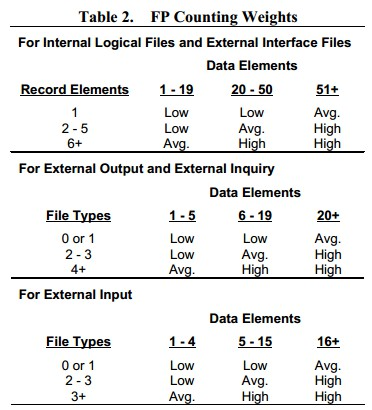
\includegraphics[width=60mm]{img/fpcounting.jpg}}
\subfigure[UFP Complexity Weights]{\label{fig:fp_total}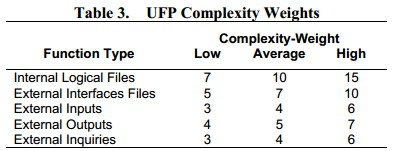
\includegraphics[width=60mm]{img/fptotal.jpg}}
\caption{FP Analysis}
\end{figure}

For each point a \textbf{counting weight} (\emph{Low}, \emph{Avg.} or \emph{High}) has been given according to the parameters specified in Figure~\ref{fig:fp_counting}. After that, a certain amount of FPs has been calculated for each section according to Figure~\ref{fig:fp_total}.

Finally, starting from the total amount of FP, we estimated the project size in SLOC (for more on this, see Section~\ref{sub:results}).

\subsection{Internal Logic Files} % (fold)
\label{sub:ilf}
The application must handle information about the following entities:

\begin{table}[h]
    \label{tab:ilf}
    \centering
    \resizebox{1\textwidth}{!}{
    \begin{tabular}{p{5cm}|cccc}
    \hline

    \hline
    \textbf{File} & \textbf{Record Elements} & \textbf{Data Elements} & \textbf{Counting Weight} & \textbf{FPs} \\
    \hline
        Customer   &   6+     &   51+     &   High    &   15 \\
        Ride       &   6+     &   51+     &   High    &   15 \\
        Call       &   6+     &   51+     &   High    &   15 \\
        TaxiDriver &   6+     &   51+     &   High    &   15 \\
        Address    &   2--5     &   51+     &   High    &   15 \\
        Zone       &   2--5     &   1--19     &   Low    &   7 \\
    \hline
        \textbf{TOT}    &   &   &   & \textbf{82} \\
    \hline
        
    \end{tabular}}
\end{table}

\subsection{External Interface File} % (fold)
\label{sub:eif}
The application must store these information from the external environment:

\begin{table}[h]
    \label{tab:eif}
    \centering
    \resizebox{1\textwidth}{!}{
    \begin{tabular}{p{5cm}|cccc}
    \hline

    \hline
    \textbf{File} & \textbf{Record Elements} & \textbf{Data Elements} & \textbf{Counting Weight} & \textbf{FPs} \\
    \hline
        Maps    &   6+     &   51+     &   High    &   10 \\
        %PaymentInfo    &   2--5    &   51+     &   High    &   10 \\
    \hline
        \textbf{TOT}    &   &   &   & \textbf{10} \\ 
    \hline
        
    \end{tabular}}
\end{table}


\subsection{External Input} % (fold)
\label{sub:ei}
The application must guarantee the following operations for the external environment:

\begin{table}[h]
    \label{tab:ei}
    \centering
    \resizebox{1\textwidth}{!}{
    \begin{tabular}{p{5cm}|cccc}
    \hline

    \hline
    \textbf{Operation} & \textbf{Entities involved} & \textbf{Data Elements} & \textbf{Counting Weight} & \textbf{FPs} \\
    \hline
        Login/signup/logout    &   1     &   16+     &   Avg    &   $3 \times 4$ \\
        Edit/delete profile    &   1     &   16+     &   Avg    &   $2 \times 4$ \\
        Add/delete request/res   &   3   &   16+     &   High    &   $3 \times 6$ \\
        Add/remove/update ride           &    1    &    16+  &  Avg & $3 \times 4$ \\
        Set   taxi status                      &     1    &   16+ &   Avg &   4 \\
        
    \hline
       \textbf{TOT}    &   &   &   & \textbf{54} \\
    \hline
        
    \end{tabular}}
\end{table}

\subsection{External Inquiry} % (fold)
\label{sub:eiq}
The application must make these inquiries available:

\begin{table}[h]
    \label{tab:eiq}
    \centering
    \resizebox{1.1\textwidth}{!}{
    \begin{tabular}{p{5cm}|cccc}
    \hline

    \hline
    \textbf{Operation} & \textbf{Entities involved} & \textbf{Data Elements} & \textbf{Counting Weight} & \textbf{FPs} \\
    \hline
        Get   previous rides    &   2     &   20+     &   High    &   6 \\
        Show  call for a user                &   3      &  20+       & High  & 6 \\
        Check existence of a ride           &   1       &   20+     & Avg   & 4 \\
        Get   info for a ride                 &   1       &   20+     & Avg   &   4 \\  
        Get   pre-calculated fee              &   1       &   20+     &   Avg &   4  \\
    \hline
       \textbf{TOT}    &   &   &   & \textbf{24}\\
    \hline
        
    \end{tabular}}
\end{table}

\subsection{External Output} % (fold)
\label{sub:eo}
The application produces data to the external environment through the following operations:

\begin{table}[h]
    \label{tab:eo}
    \centering
    \resizebox{1.1\textwidth}{!}{
    \begin{tabular}{p{5cm}|cccc}
    \hline

    \hline
    \textbf{Operation} & \textbf{Entities involved} & \textbf{Data Elements} & \textbf{Counting Weight} & \textbf{FPs} \\
    \hline
        Notification to drivers (accepting/refusing ride)              &   2 (Ride \& Customer)       &   20+     &   High &   7  \\
        Notification to customers (ride accepted)           &   2 (Ride \& Taxi)            &   20+     &   High    & 7 \\
        Confirmation email (after signup)             &       1                           &   20+     &   Avg     & 5 \\
    \hline
       \textbf{TOT}    &   &   &   & \textbf{19} \\
    \hline
        
    \end{tabular}}
\end{table}

\subsection{Results} % (fold)
\label{sub:results}
% >>>>>>>> TODO: così siamo a 189, mi sembra veramente tanto. DA RIVEDERE
According to \cite{bib:fp}, the following holds for J2EE:
\begin{equation}
    \frac{\mbox{SLOC}}{\mbox{FPs}} = 46
\end{equation}

If we sum all the results we got from the previous sections and multiply it by 46, we get ??? lines of code.
% DIRE quanto giusto / sbagliato sia questo numero di SLOC

\newpage

\section{COCOMO: effort \& cost estimation}
\subsection{Overview} % (fold)
\label{sub:cocomo_overview}
% http://www.qsm.com/resources/function-point-languages-table

\subsection{Scale Drivers} % (fold)
\label{sub:scale_drivers}

\subsection{Cost Drivers} % (fold)
\label{sub:cost_drivers}

% subsection cost_drivers (end)
% subsection scale_drivers (end)
\subsection{Effort Equation} % (fold)
\label{sub:effort_equation}

\newpage

%!TEX root = planning.tex
\section{Tasks \& Schedule}
% COMANDO PER TASK

The main tasks of this project are the following:
\begin{enumerate}
    \item Creation of the \emph{Requirement Analysis and Specification Document}, which explain in dtail functional and nonfunctional requirements, domain assumption and goals of the application to be built.
    \item Creation of the \emph{Design Document}, which deals with the architecture and the design shape of the application.
    \item Creation of the \emph{Integration Testing Plan Document}, containing the strategy to perform integration testing on the system.
    \item Creation of the \emph{Project Plan}, which is this document.
    \item Preparation of a quick presentation, using slides, (\~15 min) of the previously mentioned documents to our client.
    \item Developement of the entire application and the preparation of the unit tests.
    \item Running of integration testing on the application.
\end{enumerate}

The development of the appliction started after the creation of the Design Document and will be carried on in parallel with the rest of the tasks.  


\newpage

%!TEX root = planning.tex
\section{Resource Allocation}
% RICHIAMA CONTATORE TASK

\newpage

%!TEX root = planning.tex
\section{Risks}
Risks have to considered in a complete project planning, owing their uncertain ad dangerous nature. A sudden change in mind, actions, economical situations and alike could drift the project development into failure; this is the reason they are here analyzed. Three main risk categories will be later described:
\begin{itemize}
    \item \textbf{Project risks}: involving the \emph{project plan} (described in these pages). Project schedule and overall costs may be subject to (worse) changes due to these risks.
    \item \textbf{Technical risks}: involving the actual \emph{implementation} of the project. They may affect the quality of the software being developed.
    \item \textbf{Business risks}: involving the \emph{company} developing the software. This may cause trouble to the project (e.g. if the business cannot subsidize the software being developed anymore).
\end{itemize}

\subsection{Project Risks}

\begin{itemize}
    \risk{No estimations/schedules have been made before this project. A lack of experience in this area can lead to serious errors in evaluating development time}{High}{Critical}{Studying previous works on a similar subject can be very helpful in this.}
    \risk{Due to several overlapping tasks the team is involved into, the project is very likely to suffer from schedule delays}{High}{Critical}{A strict organization among the team components is fundamental. This implies a constant cooperation between developers, in order to squeeze even the tiniest time slots available for this project.}
    \risk{A sudden growth in requirements can lead to a rush to meeting deadlines, jeopardizing the overall quality}{Medium}{Critical}{Thinking with a broader mind on the first stages can be very helpful; however, the team should be careful against over-engineering (which can also paralyze the development)}
    \risk{Collaboration issues can sometimes be crucial, especially when dealing with task divisions.}{Medium}{Medium}{Meeting often can be a solution, other than explicitly writing who has to do what}
    \risk{The team is very small (3 people) but homogeneous; if someone leaves or gets ill then the remaining team will have serious repercussions.}{Low}{Catastrophic}{All team members must be able to cover all development sections and cooperate effectively.}
\end{itemize}

\subsection{Technical Risks}

\begin{itemize}
  \risk{A lack of previous experience in developing with Java EE can almost surely slow down the entire team, which has to study these new technologies first}{High}{Critical}{BOH}
  \risk{If the servers happen to be unreliable or in the case of more users than expected, a significant downtime can seriously damage the whole project}{Medium}{Critical}{A scalable design of the overall architecture is essential, both in software and in hardware choices.}

  % troppi accessi
  % problemi di sicurezza 
  % unit testing e integration testing
\end{itemize}


\subsection{Business Risks}

\begin{itemize}
    \risk{Testing devices \& infrastructure (PCs, several mobile phones, server rent) need to be purchased and configured. This is going to increase costs, that may be not sustainable if the company is too small.}{High}{Catastrophic}{BOH}
    % problemi finanziari
    % cambiano le leggi che regolano il servizio taxi
    % l'azienda viene acquisita
\end{itemize}

\subsection{Summary}

\appendix

\clearpage
\addcontentsline{toc}{section}{References}

\begin{thebibliography}{9}
\bibitem{bib:assignment}
    Prof. Di Nitto - \emph{Assignment 5 - Project Plan}

\bibitem{bib:rasd}
        Albanese Michele, Bianchi Mattia, Carlucci Alain - \emph{myTaxiService: Requirements Analysis and Specification Document}

\bibitem{bib:dd}
        Albanese Michele, Bianchi Mattia, Carlucci Alain - \emph{myTaxiService: Design Document}

\bibitem{bib:cid}
        Albanese Michele, Bianchi Mattia, Carlucci Alain - \emph{myTaxiService: Code Inspection Document}

\bibitem{bib:itpd}
        Albanese Michele, Bianchi Mattia, Carlucci Alain - \emph{myTaxiService: Integration Test Plan Document}

\bibitem{bib:meteocal}
        Andrea Bignoli, Leonardo Cella - \emph{MeteoCal - Project Report}

\bibitem{bib:meteocal2}
    Federico Migliavacca, Leonardo Orsello - \emph{MeteoCal - Project Reporting}

\bibitem{bib:fp} QSM - \emph{Function Point Languages Table} \small{(\url{http://www.qsm.com/resources/function-point-languages-table})}

\end{thebibliography}

\vfill

\section*{Hours spent}
Each member has spent 10 hours while writing this document.

\end{document}
